\documentclass[12pt]{article} 
\usepackage{amsmath} 
\usepackage[dvips]{graphicx}
\usepackage{multirow,multicol} 
\usepackage{geometry} 
\usepackage{pdflscape}
\usepackage[labelfont=bf]{caption} 
\usepackage{setspace}
\usepackage[running]{lineno} 
% \usepackage[numbers,sort]{natbib}
\usepackage[sort]{natbib} 
\usepackage{array}
\usepackage[table]{xcolor}
\usepackage{xr}

\newcommand{\methods}{\textit{Materials \& Methods}}
\setcounter{section}{0}
\renewcommand{\thesection}{S\arabic{section}}
\setcounter{table}{0}
\renewcommand{\thetable}{S\arabic{table}}%
\setcounter{figure}{0}
\renewcommand{\thefigure}{S\arabic{figure}}%
\setcounter{equation}{0}
\renewcommand{\theequation}{S\arabic{equation}}
\renewcommand{\labelenumi}{S\arabic{enumi}}


\topmargin -1.5cm % 0.0cm 
\oddsidemargin 0.0cm % 0.2cm 
\textwidth 6.5in
\textheight 9.0in % 21cm
\footskip 1.0cm % 1.0cm

\usepackage{authblk}

\begin{document} 

\title{Species motif participation provides unique information about species risk of extinction: supplemental information}

\author{Alyssa R. Cirtwill$^{1*\dagger}$, Anna \r{A}kesson$^{2*}$, Kate L. Wootton$^{3}$, Anna Ekl\"{o}f$^{2}$} 
\date{
\small$^1$Spatial Foodweb Ecology Group\\
Research Centre for Ecological Change\\
Organismal and Evolutionary Biology Research Programm\\
Faculty of Biological and Environmental Sciences\\
University of Helsinki, Helsinki, Finland\\
\medskip
\small$^2$Department of Theoretical Biology, Chemistry, and Physics\\ 
Link\"{o}ping University, Link\"{o}ping, Sweden\\
\medskip
\small$^3$ BioFrontiers Institute\\
University of Colorado, Boulder, Boulder, U.S.A.\\
\medskip
* Joint first authors\\
\medskip
$^\dagger$ Corresponding author\\
}


\maketitle 
\raggedright

\setlength{\parindent}{15pt} 
\begin{spacing}{2.0}

\clearpage

\section*{Table of contents}
    {\footnotesize
    \begin{spacing}{1.0}

    Appendices S1-S4 provide supplemental methods, while appendices S4-S7 provide supplemental results.

    \begin{enumerate}
    
        \item Network creation \\
        
            \begin{itemize}
            \item Construction of simulated networks
            \item Filtering of biologically unrealistic networks 
            \item Conversion of networks to acyclic form
            \item Comparison of empirical and simulated networks (Fig. S1)
            \end{itemize}
            
            
        \item Calculating persistence

            \begin{itemize}
                \item Details on functional response of consumers (Eqn. S1)
            \end{itemize}    
            

        \item Supplemental statistical analysis

            \begin{itemize}
                \item GLMs relating persistence and other network properties (Eqn. S2-S3)
                \item GLMs relating motif participation, profiles and network properties (Eqn. S4-S6)
            \end{itemize}
                
        \item Motif-persistence relationships vary with S, C

            \begin{itemize}
                \item GLMs summarising how the relationship between motif participation and persistence varies over S and C, to complement the within-network results presented in the main text (Eqn. S7)
                \item Plots of these GLMs for each motif (Figs. S2-S5)
            \end{itemize}    


        \item Supplemental results: motif participation 
            \begin{itemize}
                \item Supplemental results relating species motif participation to persistence and to other network properties (S, C, in-degree, STL)
                \item Table S1-S2; Fig. S6
            \end{itemize}

    
        \item Supplemental results: persistence

            \begin{itemize}
                \item Supplemental results identifying relationships between persistence and network size, connectance, in-degree, and STL to provide context for motif relationships (Tables S3-S4).
                \item Supplemental results relating average persistence to network motif profiles (Table S5)
            \end{itemize}    

    
        \item Supplemental results: network motif profiles

            \begin{itemize}
                \item Supplemental results relating motif profiles  to network size and connectance (Table S6; FIg. S7)
            \end{itemize}


        \item Glossary    

            \begin{itemize}
                \item Definitions of network terminology used in main text (Table S7)
            \end{itemize}


    \end{enumerate}    
\end{spacing}
}
\clearpage

\linenumbers
\section{Network creation}

    \subsection{Generation of simulated networks}

        We simulated a suite of food webs based on the probabilistic niche model, which assigns predator-prey links based on the body-mass ratios between individuals of different species~\citep{Williams2000,Delmas2017}. 
        The meso-scale structure of niche-model networks closely mimics that of empirical food webs~\citep{Stouffer2007}. 
        To ensure that we captured a variety of realistic community sizes and structures, we generated networks ranging between 50 and 100 species (in steps of 10) with connectance values between 0.02 and 0.2 (in steps of 0.02). 
        The range of network sizes was chosen to reflect moderately well-sampled empirical webs while working within our computational limits, while the range of connectance values was chosen to cover that observed in most empirical food webs~\citep{Dunne2002e}.
        We generated a total of 100 networks with each combination of parameters, for a total of 6000 networks. 
        All networks were generated using the function ``nichemodel'' within the Julia language package \emph{BioEnergeticFoodWebs}~\citep{bioenergeticfw,Delmas2017}. 
        If a simulated network contained any disconnected species (species without predators or prey) or disconnected components (a group of species connected among themselves but not to the rest of the network), the network was rejected and a new network simulated.
        Finally, networks where the path lengths between each species and a basal resource could not be resolved (i.e., trophic levels were undefined) were rejected, as was any network where any species had a shortest trophic level \textgreater6 as such high trophic levels are very uncommon in empirical food webs ~\citep{Riede2011}.
        Rejected networks were replaced with fresh simulations.


        As a further check that our simulated networks are realistic (e.g., could plausibly retain all species), we simulated community dynamics for 500 timesteps and discarded any networks which did not retain all species. 
        We simulated dynamics using the function ``simulate'' from the Julia language package \emph{BioEnergeticFoodWebs}~\citep{bioenergeticfw,Delmas2017}.
        This function uses Lotka-Volterra predator-prey models including density dependence and type 2 functional responses for all species (please see~\citet{Delmas2017} for full details).
        All non-basal species were designated as vertebrates to ensure a good match between metabolic and predator-prey body-mass ratio values. Metabolic rates in the Lotka-Volterra model are based on each species' body mass (i.e. mass of a single individual). 
        We assigned relative body masses based on each species' trophic level, which was, in turn, calculated based on the food-web structure provided by the niche model. 
        After basal species were assigned a body mass of 1, we used a predator-prey body-mass ratio of 3.065 to calculate the relative body masses of higher trophic levels. 
        We selected this ratio based on the estimate for vertebrates (averaged across ecosystem and metabolic types) in~\citet{Brose2006}. 
        We excluded reported body-mass ratios for invertebrates as these could include parasites and parasitoids, which are generally smaller than their prey, and because interactions among vertebrates are better represented in the food-web literature than interactions involving invertebrates.
        
        
        The persistence of each species in our simulated networks also depends on its population biomass. 
        We randomly assigned initial population biomasses (i.e. cumulative biomass across all individuals of a species) for each species from a uniform distribution [0,1]. 
        Note that population biomasses and individual body masses are not calculated on the same scale. 
        We then simulated community dynamics for 1000 time steps to obtain an `equilibrium' community. 
        To ensure that species did not `recover' from unrealistically low biomasses during the simulation, we considered a species extinct if it dropped below an arbitrary threshold biomass of 1$\times10^{-5}$. 
        We rejected any network where one or more species dropped below this biomass threshold. 
        Consumers were assumed to have no preferences such that the consumption rate $w_{ij}$ of predator $i$ eating prey $j$ is equal to $\frac{1}{n}$, where $n$ is the number of prey for predator $i$. 
        If the network did not retain all species for 1000 time steps, a new set of initial population biomasses was applied and the simulation repeated.
        If a set of biomasses where all species persist still had not been reached after 100 sets of randomly-assigned initial biomasses, we discarded the network and simulated another to replace it.
        
    

    \subsection{Conversion of networks to acyclic form}

        A Bayesian food web depicts probabilistic relationships among a set of species where each species' probability of persistence depends upon the probabilities of its resource species persisting~\citep{Jensen_Nielsen,Eklof2013}. 
        All persistence calculations therefore begin by determining the status of the basal resources (who do not depend on other species).
        Calculations continue in a strictly bottom-up manner with primary consumers (who depend only on basal resources), then herbivores, and so on up the network.

            
        While niche-model food webs can contain cycles (e.g., species A eats B, B eats C, and C eats A), such cycles make it impossible to calculate persistence in the Bayesian network framework~\citep{Tarjan1972}. 
        We therefore removed any cycles within each network by removing the link in each cycle which contributed least to the robustness of the food web, following~\citet{Allesina2009functional}.
        This is achieved by first finding the set of resources for each consumer and then removing the consumer-resource connections which have the lowest eigenvalue centrality~\citep{Allesina2009functional}.
        These links have the least effect on the overall stability of the network; removing them creates an acyclic network with very similar properties to the original network.
        Next, we ordered the species from lowest to highest trophic level using a topological sorting routine following \citet{Tarjan1972} and \citet{Allesinaetal2005}, ensuring that probability calculations follow a strict bottom-up order. 
        After these steps, calculations of persistence probabilities can begin.
        

    \subsection{Comparison of empirical and simulated networks}
    
        Although previous work has shown that the niche model replicates the motif structure of empirical networks~\citep{Stouffer2005a,Stouffer2006}, we additionally provide a comparison of the motif profiles and consumer motif participation for our simulated networks and the highest-quality empirical networks we could find within the same size range.
        For this comparison, we obtained all networks containing 50-100 species from \citet{globalwebdb}.
        We then removed networks where sets of predators and prey were completely different (i.e., bipartite networks) or links were not clear (i.e., +/- effects rather than predation specifically).
        This yielded five vertebrate-dominated food webs describing the California coast in different years, four invertebrate-dominated food webs describing mainland US streams, 23 invertebrate-dominated food webs describing New Zealand streams, and five other invertebrate-dominated food webs.
        This final set of webs had 50-77 species and connectances (after rendering the networks acyclic) of 0.095-0.227 - covering the upper half of the connectance range we simulate, as well as slightly higher connectances.
        This may be partly due to relatively poor resolution of basal resources in these empirical webs: aggregation of many taxa into nodes such as `phytoplankton' will tend to decrease the number of species but leave the number of links unchanged, raising connectance.
        We note that most of these webs were compiled by just three research groups.
        Moreover, many of the webs are repeated samples of the same site  or closely-grouped sites.
        This means that these empirical networks cannot be considered fully independent samples.
        
        
        \begin{figure}
            \centering
            \includegraphics[width=\textwidth]{figures/motif_profiles_participation_vs_empirical.eps}
            \caption{\textbf{A)} Proportions of acyclic motifs in the motif profiles of empirical and simulated networks. Mean proportions ($\pm$SD) in the simulated networks are indicated in black, with the range of proportions in the simulated networks indicated by black boxes. \textbf{B)} Proportions of acyclic motifs in the motif participation vectors of consumers in simulated and empirical networks.}
            \label{empirical_compare}
        \end{figure}
        
    \subsubsection{Comparing motif profiles}
    
      The proportions of omnivory and apparent competition in the motif profiles of simulated networks matched those of the empirical webs fairly well, but many of the empirical webs had higher proportions of direct competition and lower proportions of the three-species chain than any simulated web.
      The empirical webs with high proportions of direct competition tend to be invertebrate-dominated webs representing small streams.
      High proportions of direct competition in these system suggest large numbers of fairly generalist herbivore/detritivores, with relatively few secondary consumers present to create chains.
    
    
      A few webs had lower proportions of apparent competition than any simulated web but similar proportions of the other motifs.
      Most of these webs represented the California coast in different years (2003-2007).
      Basal resources in these webs were highly aggregated into only two size classes of phytoplankton and three types of detritus.
      This aggregation at the basal level leads to artificial ``specialisation'' in consumers with low trophic levels who may consume, for example, many species of phytoplankton that are grouped into a single size class.
      As the basal resources in our simulated networks are not aggregated, our webs feature higher proportions of apparent competition as seen in the other empirical webs.
    
    
    \subsubsection{Comparing motif participation}
      
      Despite the differences in network motif profiles between some of the empirical food webs and the simulated webs, we note that the motif participation of consumers in the simulated webs entirely spans the range of motif participation for consumers in the empirical webs.
      Consumers in the NZ stream food webs had higher proportions of direct competition and lower proportions of apparent competition than the mean of the simulated webs, consistent with the network motif profiles.
      Nonetheless, the greater differences in network profiles than consumer motif participation suggests that the largest differences between the simulated and empirical networks are in the roles of basal resources.
      In empirical webs, basal resources are often highly aggregated. 
      Improved resolution at the basal level should improve the correspondence between simulated and empirical webs and allow better modelling of empirical communities.
    

\clearpage        

        
\section{Calculating persistence}        

        We use Bayesian network modelling to calculate the persistence of each species in our simulated networks. 
        A Bayesian network represents a graphical model for probabilistic relationships among a set of variables. 
        In our ecological setting, the nodes of the network represent species and links represent feeding interactions between species.
        In network-theory terms, the species are Bernoulli random variables and the links represent conditional dependencies among these variables. 
        Each node has a set of local probability dependencies that are conditional on the state of the parent (resource) nodes. 
        Since the nodes are species, their state can be either extant or extinct.
        The extinction probability of each species is therefore a function of the state of its resources and also depends on a baseline probability of extinction ($\pi$) representing risk of extinction due to factors unrelated to network structure.
        In our baseline scenario, basal resources had a baseline extinction probability of $\pi = 0.1$. 
        We also simulated a set of scenarios where basal resources had a higher baseline probability of extinction ($\pi$). 
        These scenarios reflect threats to basal resources such as increased temperatures resulting in droughts, making some species more vulnerable to extinction.
        $\pi$ ranged between $0.1-0.5$, in steps of $0.08$. 
        The highest disturbance level, $\pi = 0.5$, corresponds to basal species having a 50\% risk of going extinct. 
        Consumer species retained $\pi=0.1$ in all cases.


    \subsection{Functional response of consumers}

        The response of a consumer to the loss of a fraction of its resources can be modelled in several biologically plausible ways: i) a topological response, where the consumer's probability of extinction is constant unless all resources are lost, ii) a linear response, in which the extinction probability increases linearly with resources loss, and iii) several nonlinear responses where the probability of extinction increases non-linearly with the fraction resource lost. 
        The extinction probability will differ depending on the response function.
        
        
        A sigmoid non-linear functional response of consumers to the loss of resources ($\alpha >1, \beta >1$) has been shown to most accurately capture the secondary extinctions produced by a dynamical model~\citep{Eklof2013}.
        Therefore, we use a cumulative density function of a beta distribution to get each species \textit{i} probability of extinction:
        \begin{equation}
        \label{betafunc}
        P(\lnot i|f) = \pi + (1 - \pi) \frac{B(f;\alpha,\beta)}{B(\alpha,\beta)}
        \end{equation}
        

        \noindent If all resource species of a consumer \textit{C} are present ($f = 0$), the extinction probability will be $P(\lnot C|f) = \pi$. 
        Similarly, if all resources are extinct ($f = 1$), the extinction probability $P(\lnot C|f)$ will be equal to 1 and the consumer will go extinct.
        If the fraction $f$ is not 1 nor 0, the non-linear sigmoid curve will determine the response of the consumer, which will be more severe if the fraction resources lost is high and less severe if the fraction is small. 
        This will in turn affect the extinction probability $P(\lnot C|f)$. 
        For a basal species, we assume that abiotic resources are always available. 
        Therefore, a primary producer is independent of resource species and will always have $f = 0$.  
        

        As consumer species depend on their resources, we start by determining the status of each primary producer in the network.
        Systematically, we use Equation \ref{betafunc} to calculate each species' probability of extinction $P(\lnot i|f)$, and then perform Bernoulli trials to determine whether the species goes extinct or not. 
        Imagine a basal species \textit{A} with extinction probability $P(\lnot A) = \pi$ where $\pi = 0.1$. 
        We draw a random number $r$ from a uniform distribution between $0-1$.
        The basal species would be considered extinct if $r < 0.1$ and extant otherwise. 
        
        
        We then insert the simulated fraction of species lost into Equation \ref{betafunc} to calculate $P(\lnot C|f)$ for the consumer species \textit{C}. 
        In the same manner as for the basal species above, we compare $P(\lnot C|f)$ with a random number $r$, and if $r < P(\lnot C|f)$ the consumer species is considered extinct. 
        In this way, we evaluate each species existence, starting from the bottom and working our way up.
        
        
        As this method is probabilistic, we repeat these calculations 100 000 times per network, with unique random draws.
        For each species, we then estimate the fraction of simulations in which the species persist, and this value is the approximated probability of persistence.
        To approximate persistence probabilities through numerical simulation are shown to be highly efficient and produce the same result as exact methods of solving Bayesian networks \citep{Haussler2020}.
        
        
\clearpage



\section{Supplemental statistical analysis}

    \subsection{Persistence, degree, and trophic level}
    
            In-degree and trophic level are known to influence persistence in many cases and these effects, in combination with differences in mean persistence across networks with different global properties, should also be taken into account when considering relationships between motif participation and persistence.
            To establish this necessary context, we fit GLMs with binomial error distribution:

            \begin{spacing}{1.0}
            \begin{multicols}{2}
            \begin{equation}
                    \Psi_{ink} \approx \delta_{i} + \pi_{k} + \delta_{i}\pi_{k},
                    \label{degeq}
                \end{equation}
        
            \begin{equation}
                    \Psi_{ink} \approx \tau_{i} + \pi_{k} + \tau_{i}\pi_{k},
                    \label{TLeq}
                \end{equation}
            \end{multicols}
            \end{spacing}
        
            \noindent where $\Psi_{ink}$ is the persistence of species $i$, belonging to network $n$, during disturbance level $k$, $\pi_k$ is the probability of extinction for a basal resource in disturbance level $k$, 
            $\delta_{i}$ and $\tau_i$ are the in-degree and trophic level of species $i$, respectively.
            We initially included random effects of network size and connectance and network identity but removed these terms in order to obtain a non-singular model.
            We centered and scaled the predictors before fitting the models.


    \subsection{Motif participation, profiles and other network properties}

        Species' motif participation may co-vary with other measures of network structure and species' roles within the network.
        To determine the relationships between motif participation and global network structure, we fit a set of four general linear models with binomial error distribution (one per motif):

        \begin{spacing}{1.0}
        \begin{equation}
            \rho_{in} \approx \Sigma_{n} + \zeta_{n} + \Sigma_{n}\zeta_{n},
            \label{partic_SC}
        \end{equation}
        \end{spacing}
        
        \noindent where $\rho_{in}$ is the frequency with which species $i$, belonging to network $n$, participates in the focal motif, $\Sigma_{n}$ is the size of network $n$, and $\zeta_{n}$ is the connectance of the network $n$.
        As above, we initially included a random effect of network identity but removed this term in order to obtain a non-singular model.
        Predictors were not centered or scaled before fitting.

       
        We fit a similar set of eight general linear models with binomial error distribution relating motif participation to in-degree or trophic level:

        \begin{spacing}{1.0}
        \begin{multicols}{2}
        \begin{equation}
            \rho_{in} \approx \delta_{i},
            \label{partic_deg}
        \end{equation}

        \begin{equation}
            \rho_{in} \approx \tau_{i},
            \label{partic_tl}
        \end{equation}
        \end{multicols}
        \end{spacing}
        
        \noindent where all symbols are as above. 
        As above, we initially included random effects of network size and connectance and network identity but removed these terms in order to obtain a non-singular model.
        These models were fit using the R~\citep{R} function `lmer' from the package \emph{lmerTest}~\citep{lmerTest}.

    		
\clearpage



\section{Motif-persistence relationships vary with S, C}

    \subsection{Supplemental methods}
    
        In case the within-network trends with respect to network size and connectance are easier to understand after summarising across all networks, we fit four general linear models with binomial error distribution (GLMs; one per motif which can occur in acyclic networks): 
             \begin{equation}
             \begin{aligned}
            \Psi_{ink} & \approx \rho_{i} + \pi_{k} + \Sigma_{n} + \zeta_{n} \\
            & + \rho_{i}\pi_{k} + \rho_{i}\Sigma_{n} + \rho_{i}\zeta_{n} + \pi_{k}\Sigma_{n} + \pi_{k}\zeta_{n} + \Sigma_{n}\zeta_{n} \\
            & + \rho_{i}\pi_{k}\Sigma_{n} + \rho_{i}\pi_{k}\zeta_{n} + \pi_{k}\Sigma_{n}\zeta_{n} + \rho_{i}\pi_{k}\Sigma_{n}\zeta_{n} ,
            % S_{n}C_{n} + N_n,
            \label{propreq}
            \end{aligned}
            \end{equation}
            \noindent where $\Psi_{ink}$ is the persistence of species $i$, belonging to network $n$, during disturbance level $k$, $\rho_{i}$ is the proportion of the role of species $i$ that is made up by the focal motif, $\pi_k$ is the probability of extinction for a basal resource in disturbance level $k$, $\Sigma_{n}$ is the number of species in the network, and $\zeta_{n}$ is the connectance of the network.
            All predictors were centered and scaled before fitting the models.    
            After fitting the full models described above, we removed any non-significant terms in a stepwise fashion, beginning with the four-way interaction and proceeding to three-way and two-way interactions.
            If a smaller term was included in a significant larger term (e.g., a non-significant two-way interaction involving terms in a significant three-way interaction) then the smaller term was retained.

    \subsection{Supplemental results}
    
    \begin{figure}[ht!]
        \centering
        \includegraphics[width=\textwidth]{figures/persistence_omnivory_detailpers.eps}
        \caption{The relationship between the proportion of omnivory in the participation vector and probability of persistence depended strongly on the connectance of the network.
        Higher proportions of omnivory were associated with lower probabilities of persistence when connectance was low, regardless of network size or strength of disturbance.
        At moderate connectance, however, higher proportions of omnivory were associated with greater probabilities of persistence when disturbance was weak.
        In the most-connected networks, higher proportions of omnivory were associated with greater probabilities of persistence at all levels of disturbance.}
        \label{omnivory_plus_SC}
        \end{figure}

    \begin{figure}[hb!]
        \centering
        \includegraphics[width=\textwidth]{figures/persistence_chain_detailpers.eps}
        \caption{The relationship between proportion of the three-species chain in the participation vector and persistence was very similar across all levels of size and connectance.}
        \label{chain_plus_SC}
        \end{figure}

    \begin{figure}[hb!]
        \centering
        \includegraphics[width=\textwidth]{figures/persistence_apparent_detailpers.eps}
        \caption{Slopes of the motif proportion-persistence relationships for the apparent competition motif were steepest in large and less-connected networks or small and highly-connected networks but the directions of slopes varied only with the strength of disturbance.}
        \label{apparent_plus_SC}
        \end{figure}

    \begin{figure}[hb!]
        \centering
        \includegraphics[width=\textwidth]{figures/persistence_direct_detailpers.eps}
        \caption{Slopes of the motif proportion-persistence relationships for the direct competition motif were steepest in less-connected networks but the directions of slopes varied only with the strength of disturbance.}
        \label{direct_plus_SC}
        \end{figure}
    

\clearpage


\section{Supplemental results: motif participation} 

    \subsection{Participation and persistence}


    % Updated with new random effect, converted to data-scale
    \begin{table}[ht!]
        \centering
        \caption{Coefficients ($\beta$) for general linear models relating persistence to the proportion of a species' role made up by the focal motif, the level of disturbance to basal resources (corresponding to a probability of extinction ranging between 0.1 and 0.5), and their interaction  (Eq. 1, main text). Coefficients in \textbf{bold} are significant ($\alpha$\textless0.005). Models were fit using a binomial error distribution and logit link function. Predictors were centered and scaled before model fitting. We also provide McFadden's pseudo-$R^2$ for each model.}
        \label{tab:proportion}                \footnotesize
        \begin{tabular}{c|c c c c | c }
        Motif & Intercept & Proportion & Disturbance & Interaction & pseudo-$R^2$  \\
        \hline
        3-sp Chain & \textbf{2.90} & \textbf{-0.204} & \textbf{-5.42} & \textbf{0.138} & 0.895 \\
        App. Com. & \textbf{0.317} & -2.63$\times10^{-3}$ & \textbf{-5.98478} & \textbf{1.95$\times10^{-2}$} & 0.895 \\
        Dir. Com. & \textbf{0.317} & \textbf{3.03$\times10^{-2}$} & \textbf{-0.599} & -1.67$\times10^{-3}$ &  0.897 \\
        Omnivory & \textbf{0.317} & \textbf{-1.81$\times10^{-2}$} & \textbf{-0.598} & \textbf{-7.76$\times10^{-3}$} & 0.895 \\
        \end{tabular}
    \end{table}        

\subsection{Participation and network properties} 


    \begin{figure}[ht!]
        \centering
        \includegraphics[width=\textwidth]{figures/roles_vs_SC_all.eps}
        \caption{The proportion of each motif in consumer's participation vectors varied with connectance, network size, and their interaction (except for apparent competition, where there was no significant interaction).}
        \label{fig:motifs_vs_TL_and_deg}
    \end{figure}    

    \begin{table}[hb!]
        \centering
        \caption{Motif participation varies with size and connectance. Here we give the range and mean proportion of each motif in species' motif participation vectors. 
        We also show the coefficients ($\beta$) for network size (S), connectance (C), and their interaction in general linear models predicting the proportion of each motif in a participation vector.
        Coefficients in \textbf{bold} are significant ($\alpha$=0.05).
        We also show the coefficients for similar models relating the proportion of each motif to in-degree or trophic level.
        All models were fit with a binomial error distribution and logit link function.
        Predictors were not centered or standardized before model fitting. Motifs are ordered according to mean proportion.}
        % Relevant lms are pchainlm, pomnilm, papplm, pdirlm}
        \label{tab:partic_vs_SC}   
        \footnotesize
        \begin{tabular}{c|c c c | c c c | c | c}
            Motif & Min & Max & Mean & S & C & Int. & in-Deg & TL \\
            \hline
            3-sp Chain & 0 & 1 & 0.249 & \textbf{1.20$\times10^{-3}$} &  -0.652 & \textbf{-1.77$\times10^{-2}$} & \textbf{-6.99$\times10^{-3}$} & \textbf{9.84$\times10^{-2}$} \\
            App. Comp & 0.250 & 0.765 & 0.422 & \textbf{-1.82$\times10^{-3}$} & \textbf{-3.18} & 6.92$\times10^{-3}$ & \textbf{-8.76$\times10^{-3}$} & \textbf{2.40$\times10^{-1}$}\\
            Dir. Comp & 0.0501 & 0.359 & 0.179 & -1.18$\times10^{-3}$ & \textbf{-4.50} & \textbf{4.79$\times10^{-2}$} & \textbf{-1.43$\times10^{-3}$} & \textbf{-2.52$\times10^{-1}$} \\
            Omnivory & 0.006 & 0.346 & 0.164 & \textbf{3.64$\times10^{-3}$} & \textbf{12.5} & \textbf{-4.19$\times10^{-2}$} & \textbf{2.29$\times10^{-2}$} & \textbf{-2.27$\times10^{-1}$}\\   
            \hline
            \end{tabular}
            \end{table}


\clearpage 

\section{Supplemental results: persistence} 

    \subsection{Persistence and non-motif measures}
    % \begin{figure}[ht!]
    %     \centering
    %     \includegraphics[width=0.9\textwidth]{figures/persistence_vs_SC_lm.eps}
    %     \caption{Persistence decreased strongly with increasing probability of disturbance to basal resources and decreased slightly, but significantly, with increasing connectance.}
    %     \label{fig:lm_CS}
    % \end{figure}

    % Updated with network-level random effect
    \begin{table}[hb!]
        \caption{Coeffcients ($\beta$) for general linear mixed-effect models of consumers' probabilities of persistence against simple measures of species' role (STL or in-degree), level of disturbance to basal resources, and their interaction, as well as a random effect of global network properties (size and connectance). The model for STL was singular when including the random effect, so we removed this term and re-fit the model as a general linear model with fixed effects only. All models had binomial error distribution. All $p$-values were \textless0.001. The level of disturbance is reflected by basal resources having a baseline probability of extinction ranging between $0.1 - 0.5$.  We also provide the marginal $R^2_M$ (fixed effects only) and conditional $R^2_C$ (fixed and random effects) for the in-degree model and the pseudo-$R^2$ for the STL model.}
        \label{tab:per_vs_TLdeg}
        \centering
        \begin{tabular}{l|c  c  c | c c  }
            Simple role measure & Role & Disturbance & Interaction & R$^2_M$ & R$^2_C$ \\
            \hline
            STL & \textbf{-0.0977} & \textbf{-0.600} & \textbf{0.0302} & \textbf{0.920} & NA \\
            in-degree & \textbf{-1.30$\times10^{-3}$} & \textbf{-0.139} & \textbf{-9.08$\times10^{-3}$} & 0.903 & 0.914 \\
        \end{tabular}
    \end{table}


    
    % Updated to use mean rather than all species.
    \begin{table}[hb!]
        \caption{Mean persistence of consumers within a network depends on connectance (C) and the level of disturbance to basal resources (D), but not network size (S) or interactions between properties. We show effect sizes ($\beta$) and $p$-values for each coefficient, except the intercept (see Appendix S3 for details). McFadden's pseudo-$R^2$=0.966. }
        \label{tab:per_vs_SC}
        \centering
        \footnotesize
        \begin{tabular}{c| c c c c c c c}
              & S & C & D & S:C & S:D & C:D & S:C:D \\
            \hline
             $\beta$ &	 -7.21$\times10^{-4}$  	& \textbf{-6.12$\times10^{-2}$}	& \textbf{-0.596} &	 -4.48$\times10^{-3}$ &	 -1.63$\times10^{-2}$ 	& -4.52$\times10^{-3}$ &	 -1.35$\times10^{-3}$ \\
             $p$-value &		 0.964 &	 \textless0.001 &	 \textless0.001 &	 0.777 &	 0.316 &	 0.781 &	 0.934 \\
                    \end{tabular}
                \end{table}



    % \begin{figure}[hb!]
    %  \centering
    %  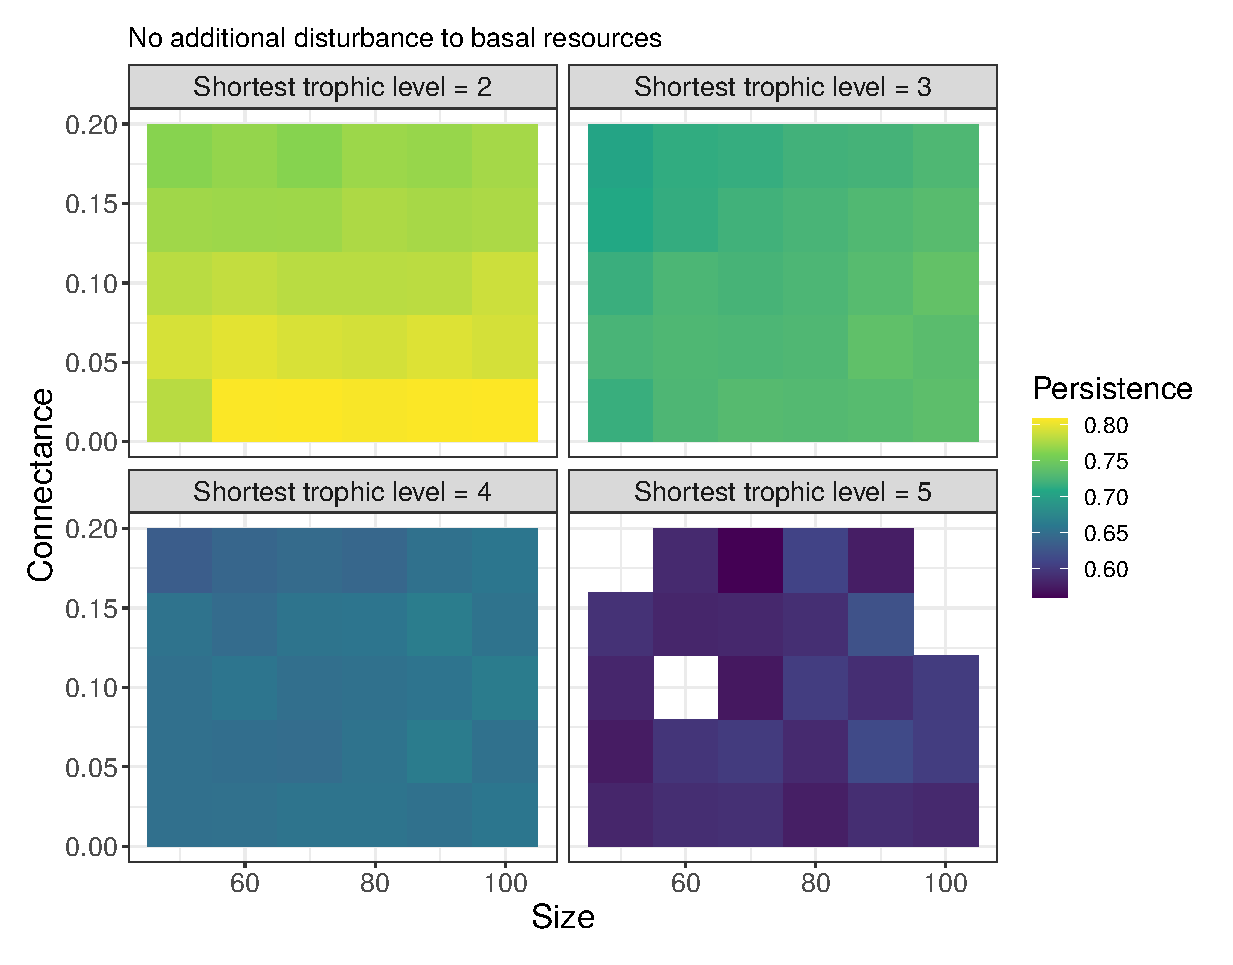
\includegraphics[width=.9\textwidth]{figures/heatmap_STL_allCS_BP0.eps}
    %  \caption{All species across all levels experience a risk of going extinct due to causes not related to the web of $\pi = 0.1$. The panels show final persistence for consumers with different shortest trophic level, for increasing connectance (y-axis) and network size (x-axis). Persistence decreases with darker color in the heat map.}
    %  \label{fig:heatmap_stl_BP0}
    % \end{figure}


    % \begin{figure}[hb!]
    %  \centering
    %  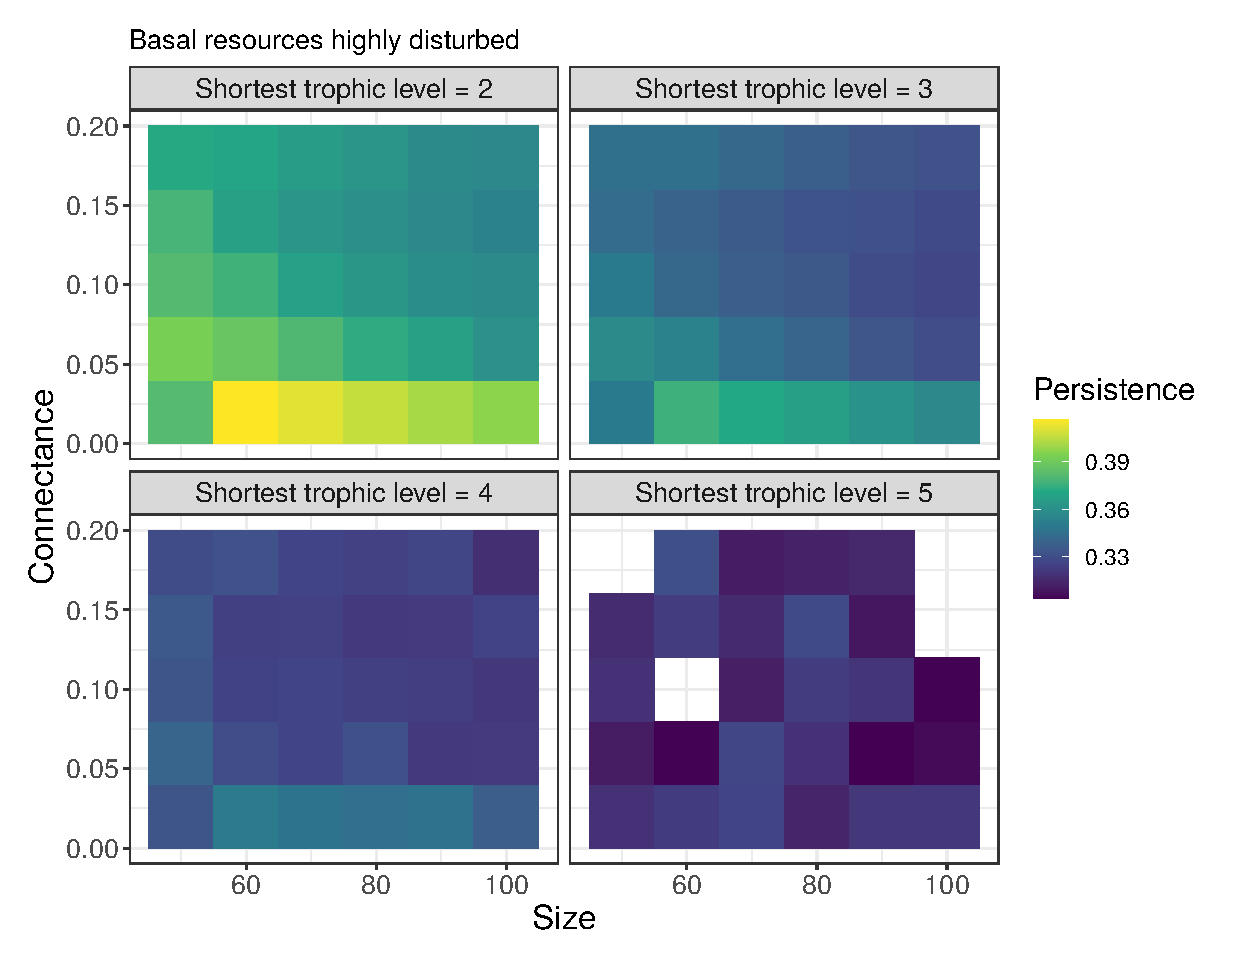
\includegraphics[width=.9\textwidth]{figures/heatmap_STL_allCS_BP1.eps}
    %  \caption{Basal resources experience a disturbance increasing their probability of extinction to $\pi = 0.5$. All consumer species go extinct due to causes not related to the web itself with probability $\pi = 0.1$. The panels show final persistence for consumers with different shortest trophic level, for increasing connectance (y-axis) and network size (x-axis). Persistence decreases with darker color in the heat map.}
    %  \label{fig:heatmap_stl_BP1}
    % \end{figure}

    \subsection{Persistence and whole-network motif profiles}


    % Updated to use mean instead of all species
    \begin{table}[ht!]
        \caption{These results correspond to equation 2, main text. Coefficients ($\beta$) for models relating persistence to the proportion of a network profile made up by a focal motif, the level of disturbance to basal resources (corresponding to a probability of extinction ranging between 0.1 and 0.5), and their interaction. Coefficients in \textbf{bold} are significant ($\alpha$\textless0.005). We also provide McFadden's pseudo-$R^2$ value for each regression. }
        \label{motif_profile_tab}
        \centering
        \footnotesize
        \begin{tabular}{c|c c c c c | c }
        Motif & Intercept & Proportion & Disturbance & Interaction &  pseudo-$R^2$ \\
            \hline
            Three-species chain & \textbf{0.326} &  0.0260 & \textbf{-0.595} & -2.53$\times10^{-3}$ & 0.958 \\
            Apparent competition & \textbf{0.326} & \textbf{0.0501} & \textbf{-0.596} & -2.00$\times10^{-3}$ & 0.962 \\
            Direct competition & \textbf{0.326} & 0.0151 & \textbf{-0.595} & -5.34$\times10^{-4}$ & 0.956 \\
            Omnivory & \textbf{0.326} & \textbf{-0.0626} & \textbf{-0.596} & 3.22$\times10^{-3}$ & 0.966 \\
        \end{tabular}
    \end{table}


\clearpage

                

\section{Supplemental results: network motif profiles}


    \subsection{Motif profiles and network size, connectance}
    % No update needed
    
        A series of general linear regressions support the relationship between network motif profiles and global structural properties.
        Specifically, the frequency of the omnivory motif increased in more-connected networks (Table~\ref{network_prop_lms}) while the frequencies of other motifs were not significantly related to network size or connectance.
    
    \begin{figure}[hb!]
        \centering
        \includegraphics[width=\textwidth]{figures/motif_proportion_lms.eps}
        \caption{The proportion of the omnivory in a network's motif role increased significantly as connectance increased, while the proportions of the other three motifs did not vary significantly with network size, connectance, or their interaction.}
        \label{motif_proportion_lms}
    \end{figure}    
    
       % \begin{figure}[hb!]
       %     \centering
       %     \includegraphics[width=.75\textwidth]{figures/proportion_profile_dispersion.eps}
       %     \caption{Dispersion of normalized motif profiles (i.e., proportions of each motif) within a network about the centroid for that combination of network size and connectance. Each circle represents a single network; circle colour indicates network size. Scatter has been introduced about each level of connectance to increase visual clarity; the levels of connectance we consider are indicated by vertical black lines.}
       %     \label{dispersion_normmotifs}
       %  \end{figure}
    
    
         \begin{table}[hb!]
            \centering
            \caption{Coefficients for general linear regressions relating the proportion of each motif in the total motif profile of a network to network size, connectance, and their interaction. Coefficients in \textbf{bold} are significant ($\alpha$\textless0.05). The regression was fit using a binomial error distribution and logit link function.}
           \label{network_prop_lms}
           \begin{tabular}{c|c c c c c}
                Motif & Intercept & Size & Connectance & Interaction \\
                \hline
                Three-species Chain & \textbf{-1.04} & 0.001 & -0.795 & -0.019 \\
                Apparent Competition & 0.168 & -0.002 & -4.09 & 0.010 \\
                Direct Competition & \textbf{-1.42} & -3.69$\times10^{-4}$ & -3.97 & 0.042 \\
                Omnivory & \textbf{-2.99} & 0.003 & \textbf{12.9} & -0.036\\
                \hline
                \end{tabular}
        \end{table}        
\clearpage
    
            




\clearpage

\section{Glossary}

 \begin{table}[hb!]
 \label{glossary}
 \caption{Glossary of terms relating to motifs and Bayesian networks}
     \footnotesize{
 \begin{tabular}{l|m{11cm}}
     Term & Definition \\
     \hline
     Global property & A property of the whole network (e.g., species richness) \\
     Local property & A property of a single species, generally referring only to direct interactions (e.g., degree) \\
     Meso-scale property &  A property of a single species which includes direct and indirect interactions; the species' immediate `neighbourhood' in the network (e.g., motif participation) \\
     Motif & Set of $n$ interacting species. In this case, $n=3$ \\
     Network motif profile & Vector describing the frequency of each motif in the network (normalised by dividing counts of each motif by the total participation in  all motifs).\\
     Motif participation role & Vector describing the frequency with which a focal species appears in each motif  (normalised by dividing counts for each motif by the total of all motifs). \\
     Bayesian network & A directed acyclic graph, used to efficiently predict species' likelihood of persistence based on the state of their resources. \\
     Network mean persistence & The mean likelihood of persistence for all consumers in a network.\\
     Species persistence & The likelihood of a particular focal species not going extinct.\\
     In-degree & Number of prey species to a consumer species.\\
     Trophic level (STL) & Length of shortest food chain between the focal species and any basal resource.\\
     Disturbance ($\pi_{disturbed}$) & Probability of extinction of a basal resource after a disturbance is added. \\
     Baseline extinction &  Probability of extinction when no disturbance is applied, $\pi_{base}$=0.1.\\
 \end{tabular}}
 \end{table}
 
\clearpage 

\bibliographystyle{jae} 
\bibliography{anna_bib_new} % Abbreviate journal titles.

\end{spacing}

\end{document}